%! TEX root = ../tor.tex

\chapter{Funcționarea, pe scurt}

\section{Relee și \qq{foi de ceapă}}
\indent\indent Într-o formă simplificată, Tor funcționează prin transmiterea conexiunii 
printr-o serie de \emph{relee} (eng.\ \texttt{relay}) de la computerul inițiator pînă la
destinație.

Actualmente, există peste 6000 de relee în toată lumea, care se ocupă cu această
redirecționare a traficului. Releele sînt localizate în întreaga lume și puse la
dispoziție de voluntari.

Într-o conexiune standard, Tor realizează conexiunea cu 3 relee, fiecare dintre
acestea avînd cîte un rol standard.
\begin{figure}[!htbp]
  \centering
  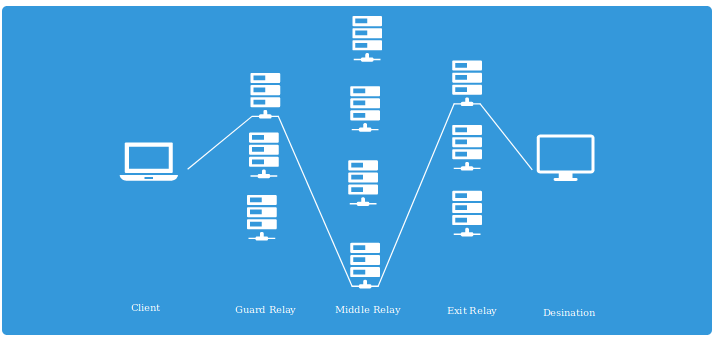
\includegraphics[scale=0.5]{fig/3relays.png}
  \caption{Cele 3 relee standard (\cite{jw1})}
  \label{fig:3rel}
\end{figure}

\begin{itemize}
  \item \textit{Releul de intrare} (eng.\ \texttt{entry/guard}), prin care conexiunea
    intră în rețeaua Tor. Asemenea relee sînt alese după ce au dovedit o vechime
    în rețea, stabilitate și lățime de bandă corespunzătoare.
  \item \emph{Relee intermediare} sînt cele care transmit conexiunea mai departe.
    Totodată, în ideea anonimizării, rolul lor este ca releele de intrare și cele
    de ieșire să nu se cunoască între ele.
  \item \emph{Releul de ieșire}, care se află la capătul rețelei Tor și trimit 
    traficul către destinația finală dorită de client.
\end{itemize}
\index{releu}
\index{releu!de intrare}
\index{releu!intermediar}
\index{releu!de ieșire}

De remarcat este faptul că, dacă releele intermediare pot fi orice calculator, server
etc., care nu se compromit în niciun fel, deoarece ele nu fac decît să transporte
trafic deja criptat, releele de ieșire au o responsabilitate deosebită. În cazul unei
conexiuni ilicite, traficul către destinație apare ca fiind transmis de la releul
de ieșire, ceea ce-i expune în mod deosebit.

La fiecare pas se realizează o decriptare, dacă traficul circulă de la client către
server și o criptare, dacă traficul circulă invers. Așa cum am menționat în secțiunea
anterioară, fiecare nod intermediar adaugă sau elimină cîte un strat criptografic,
realizînd \qq{rutarea în foi de ceapă}.

\begin{figure}[!htbp]
  \centering
  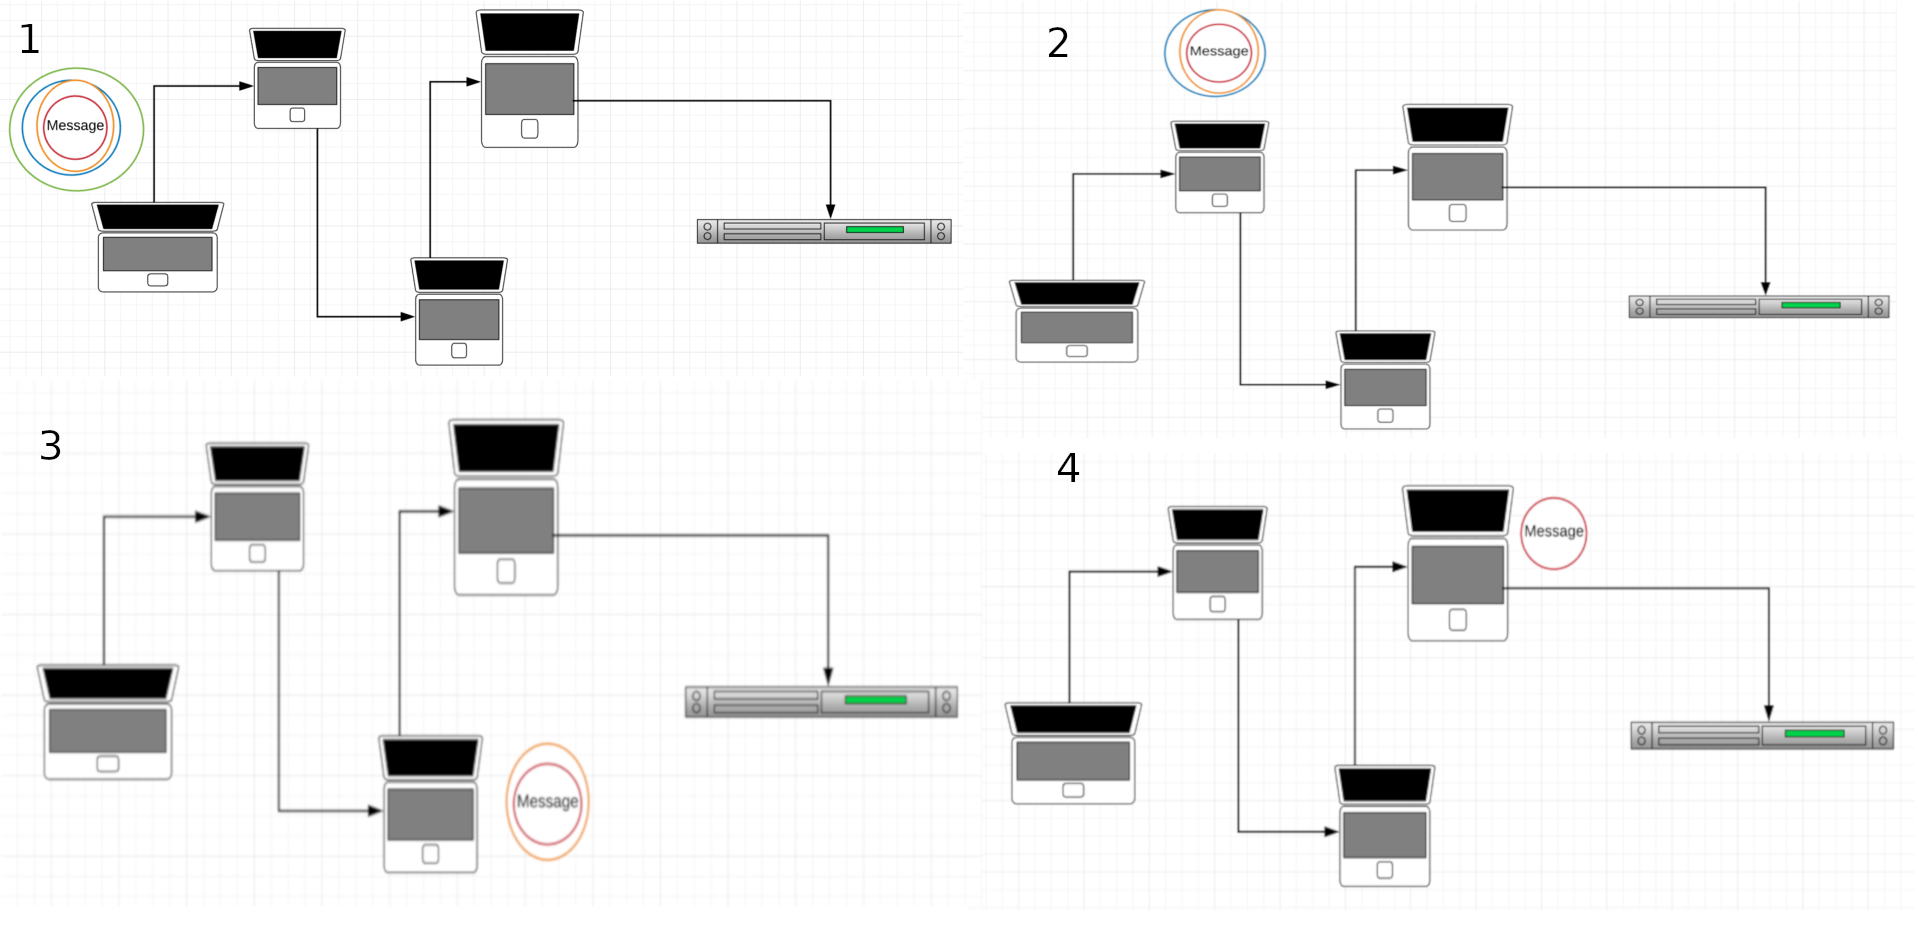
\includegraphics{fig/4onions.png}
  \caption{\qq{Foile de ceapă} (\cite{bs})}
  \label{fig:4on}
\end{figure}


Prin acest mecanism, fiecare releu cunoaște doar minimul necesar: nodul anterior și
nodul care va urma, realizînd \emph{criptarea telescopică} despre care am mai vorbit.
De remarcat este faptul că releul de ieșire vede datele inițiale trimise de client.
Astfel, dacă se trimit date sensibile prin protocoale care folosesc text clar, precum
HTTP sau FTP, releul de ieșire poate să intercepteze traficul.

%%%%%%%%%%%%%%%%%%%%%%%%%%%%%%%%%%%%%%%%%%%%%%%%%%%%%%%%%%%%%%%%%%%%%%

\section{Poduri} \index{poduri}

\indent\indent Utilizarea releelor, în forma descrisă mai sus, ridică o vulnerabilitate
serioasă. Astfel, atunci cînd un client se conectează la rețea, trebuie să aibă acces
la lista tuturor releelor de intrare, mediane și de ieșire, pentru a ști unde s-ar putea
conecta. Lista releelor nu este secretă, ceea ce ridică o potențială problemă de securitate.

O soluție pentru această problemă este utilizarea \emph{podurilor} (eng.\ \texttt{bridges}).
Într-o formă simplificată, putem privi podurile ca intrări secrete în relee, pe care le
pot accesa, de exemplu, utilizatori care se află în spatele unor rețele cenzurate.

Există și o listă completă de poduri, deținută de proiectul Tor, dar această listă
nu este publicată. Cei de la Tor au găsit o soluție prin care utilizatorii să aibă
acces doar la o porțiune mică a listei podurilor, suficiente pentru a iniția o conexiune.
Astfel, utilizatorul nici nu are nevoie de toate podurile disponibile, ci doar de cîteva
pentru a-și face intrarea în rețea.

Cercetătorii au reușit să identifice între 79\% și 86\% din lista totală a podurilor
(cf.\ \cite{jw1}), realizînd o analiză a întregului spațiu de adrese IPv4, dar 
chiar și așa, putem considera că secretul listei podurilor este suficient de bine păstrat.

%%%%%%%%%%%%%%%%%%%%%%%%%%%%%%%%%%%%%%%%%%%%%%%%%%%%%%%%%%%%%%%%%%%%%%
\section{Autorități directoare} \index{autorități directoare}

\indent\indent Am menționat în prima parte faptul că în rețea există o serie
de autorități directoare, care sînt nodurile cele mai de încredere și, într-un fel,
țin funcționare proiectului în spate.

Statusul releelor Tor este ținut într-un document dinamic, numit \emph{consens}. \index{consens}
Acest document este întreținut de autoritățile directoare (AD) și actualizat
în fiecare oră prin voturi, în următorul mod:
\begin{itemize}
  \item fiecare AD face o listă de relee cunoscute;
  \item fiecare AD calculează și ceilalți parametri necesari despre relee (țara,
    lățimea de bandă etc.);
  \item AD transmite această informație sub forma unui status celorlalte AD;
  \item fiecare AD primește acest status, din care își actualizează propria
    listă;
  \item toți parametrii adunați de la toate AD sînt combinate și se cal\-cu\-lea\-ză
    un vot, ca\-re este transmis cu o semnătură de către fiecare AD;
  \item releele care primesc majoritatea voturilor sînt păstrate în consens, ca\-re
    se actualizează și se transmite tuturor AD.
\end{itemize}

Procesul de vot și actualizare de mai sus este public, transmis prin HTTP, astfel
încît poate fi accesat de orice utilizator.


%%%%%%%%%%%%%%%%%%%%%%%%%%%%%%%%%%%%%%%%%%%%%%%%%%%%%%%%%%%%%%%%%%%%%%

\section{Servicii ascunse}

\indent\indent Un server poate fi configurat să funcționeze ca un serviciu
ascuns. Atunci cînd se realizează această configurare, serverul trimite
un mesaj către un OR ales (aleatoriu sau după o procedură specifică) pentru
a cere ca acel OR să devină punct de intrare pentru serverul respectiv.

Apoi, serverul creează un descriptor pentru servicii ascunse, care este
criptat cu o cheie publică și conține IP-urile fiecăror puncte de introducere
care a acceptat să conexiunea. Această informație este trimisă unui tabel
de hash-uri distribuit, deci fiecare OR va avea doar o parte a informației
despre serviciul ascuns. Cheia pentru acest tabel este adresa onion, care
este calculată de server.

\index{onion!adresă (hash)}
Ideea de bază este că această adresă nu este publică la nivel de rețea Tor,
ci este cunoscută doar de cei ce vor să o acceseze. Este vorba despre
adresele de tip \texttt{[hash].onion}. Deci fiecare OR are cunoștințe minime
despre aceste servicii ascunse, dar utilizatorul care vrea să se conecteze
în mod explicit, o poate face.

Atunci cînd utilizatorul cere explicit conexiunea la servicii ascunse,
introducînd a\-dre\-sa \texttt{.onion}, primește lista de IP-uri care pot servi
drept noduri de intrare către adresa respectivă. Se alege una aleatoriu
și se stabilește circuitul, folosind celulele de mărime fixată (pentru ca
un observator să nu-și dea seama, de exemplu, că celulele mai mari corespund
imaginilor sau videoclipurilor).

Pe scurt, funcționarea serviciilor ascunse urmează pașii:
\begin{enumerate}[(1)]
  \item Calculează perechea de chei pentru criptarea asimetrică;
  \item Alege un releu ca punct de introducere;
  \item Comunică cheia publică releurilor alese;
  \item Creează un descriptor specific, care conține cheia publică și 
    punctele de introducere;
  \item Scrie descriptorul într-o listă de hash-uri distribuită;
  \item Clientul află adresa de tip \texttt{[hash].onion}, obținută din
    cheia publică;
  \item Clientul se conectează la tabelul distribuit și cere să acceseze
    serviciul corespunzător hash-ului din adresa \texttt{.onion};
  \item Dacă serviciul există, clientul află cheia publică a serviciului
    și punctele de introducere;
  \item Clientul alege un punct de introducere la întîmplare și-i comunică
    un cod de tip one time. Releul ales pentru introducere joacă rol de 
    punct de întîlnire;
  \item Clientul creează o celulă de introducere, care conține adresa
    punctului de întîlnire de accesat și codul one time, pe care le criptează
    cu cheia publică a serviciului ascuns;
  \item Clientul trimite mesajul de mai sus în rețeaua Tor către punctul de
    introducere ales, cerînd să se facă legătura cu serviciul ascuns;
  \item Serviciul ascuns decriptează mesajul de introducere cu cheia privată
    pentru a obține informațiile trimise;
   \item De îndată ce serviciul ascuns descoperă punctul de întîlnire ales,
     îl transmite clientului ca fiind acceptat;
   \item Clientul și serviciul ascuns comunică folosind acest punct de întîlnire,
     avînd traficul criptat la ambele capete. Atît clientul, cît și serverul ascuns
     își creează propriul circuit pînă la punctul de întîlnire, fiecare circuit
     avînd cel puțin 3 noduri, deci o asemenea conexiune are cel puțin 6 noduri.
\end{enumerate}
\index{serviciu ascuns}
\index{server!ascuns}
